% The paired minor against adult contrast on four measures, stacked one a row.
% Chapter 4, Section 4.3.2, after Table~\ref{tab:readability-conditioning}.
%
% Stacked rather than tiled, and the reason is typographic. Each source PDF is
% 656.4pt wide and was set by styled() so that its type arrives at 11 points
% when the file is included at the full 453.5pt text block. Included at
% \textwidth that is what happens, at 10.9 points. Tiled two across at
% 0.48\textwidth the same file is scaled to a third of its canvas and the type
% arrives at about 5.2 points, which is why the two by two version of this
% figure was abandoned.
%
% Four panels at full width is 1,098pt of art against a 703pt text block, so it
% cannot be one page. It runs two to a page across two floats under one number
% via \ContinuedFloat, which is the pattern Appendix G already uses. The caption
% is given once, on the first part, so the List of Figures carries a single
% entry; the continuation takes \caption[]{} so it adds none, and that empty
% optional argument must stay or a second entry appears.
%
% The summary row in panels (b), (c) and (d) used to be a contrast over the
% pooled replies of all six models. It is now the joint bootstrap over the six
% model effects, as panel (a) has always been, so all four rows mean the same
% thing and the Note no longer has to warn that they do not.
\begin{figure}[p]
\centering

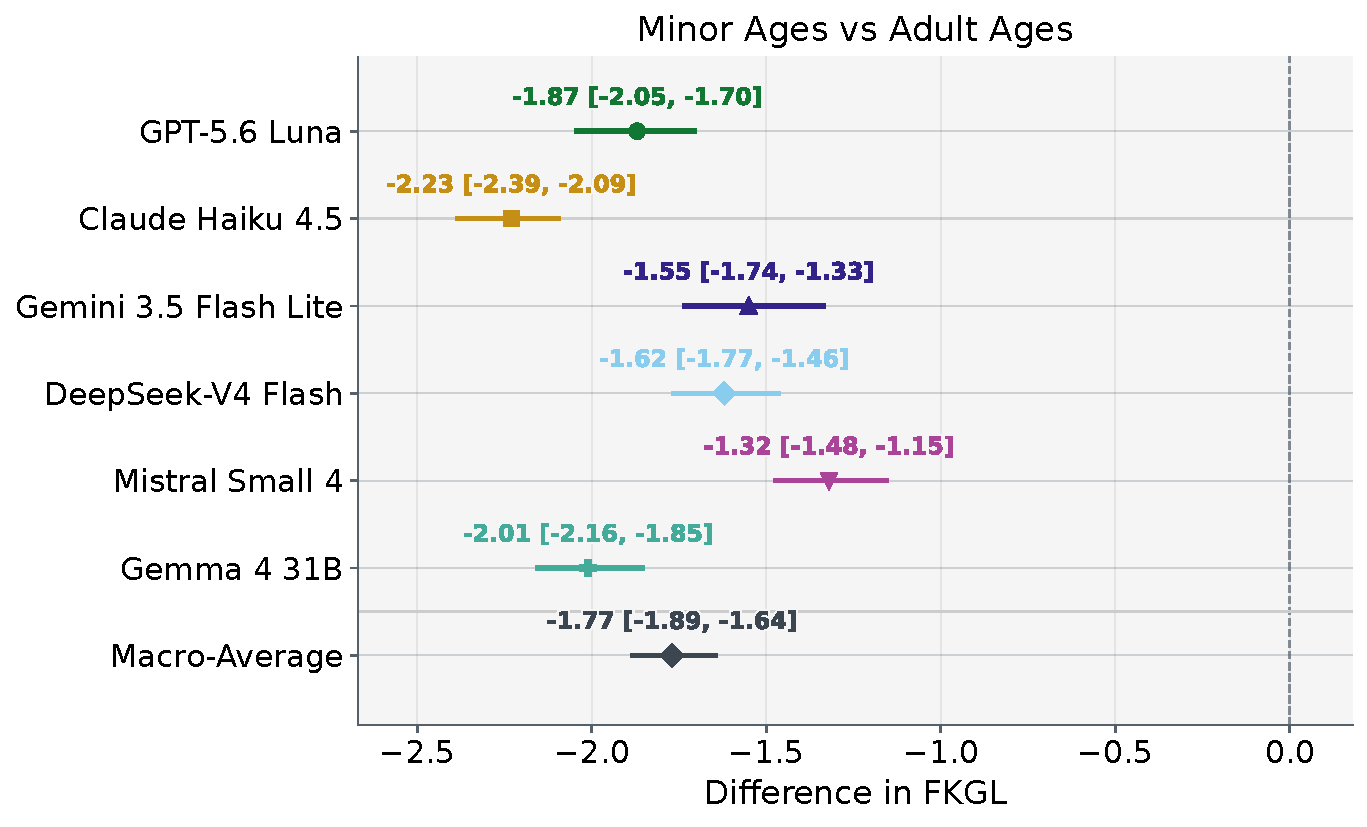
\includegraphics[width=0.6\textwidth]{read/readability_conditioning.pdf}\\[0.3em]
{\small (a) Flesch-Kincaid grade level, in school grades}

\vspace{1.4em}

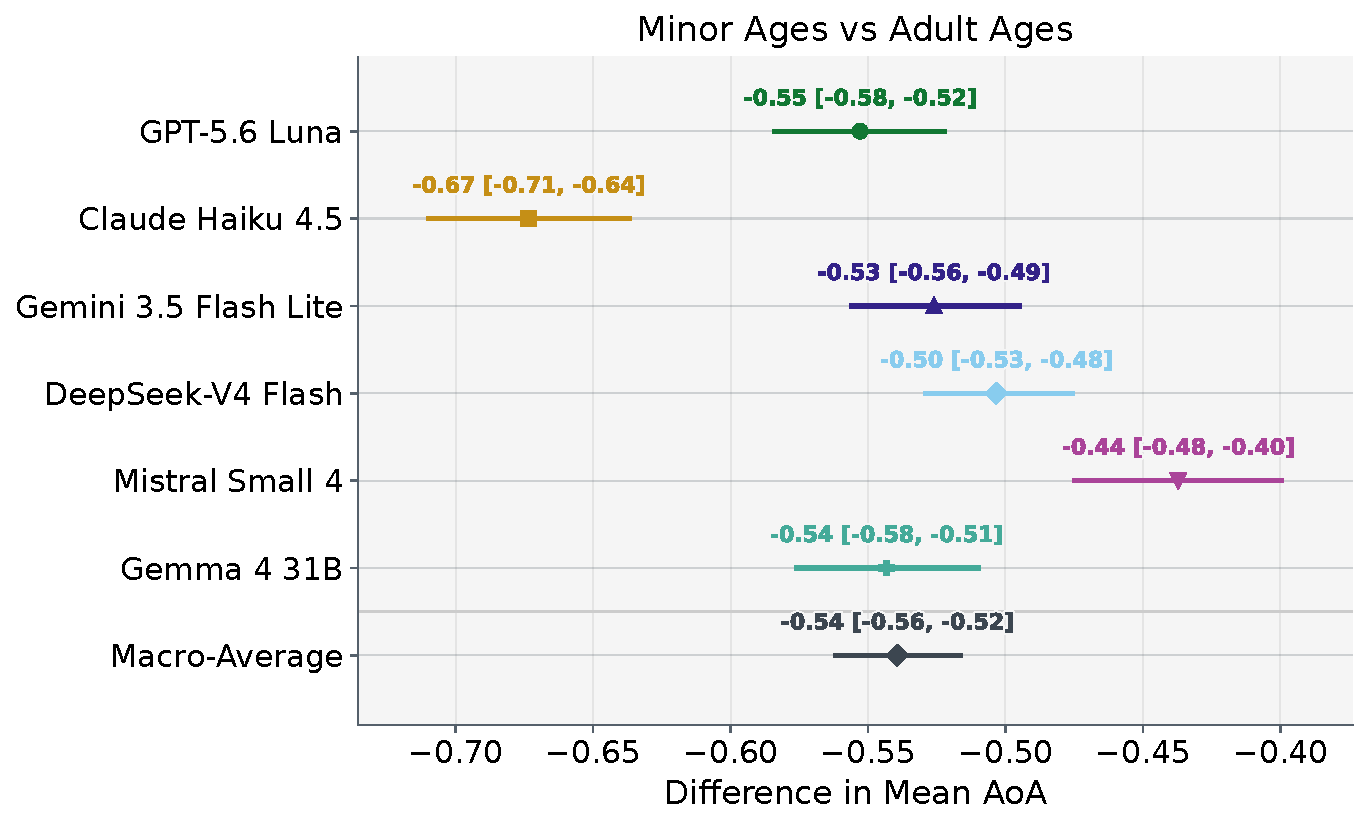
\includegraphics[width=0.6\textwidth]{read/readability_conditioning_mean_aoa.pdf}\\[0.3em]
{\small (b) Mean age of acquisition, in years}

\caption{\emph{Experiment 1} $\vert$ Four Measures by Age Contrast}
\label{fig:readability-conditioning-grid}
\vspace{0.4em}
\begin{minipage}{\textwidth}
\footnotesize
\emph{Note.} The minor against adult contrast on four language measures, paired
within scenario with 95\% bootstrap intervals. A negative effect is a lower
measure where the user gave a minor age. The summary row is the joint-bootstrap
macro-average of Section~\ref{sec:statistics}.
\end{minipage}
\end{figure}

\begin{figure}[p]\ContinuedFloat
\centering

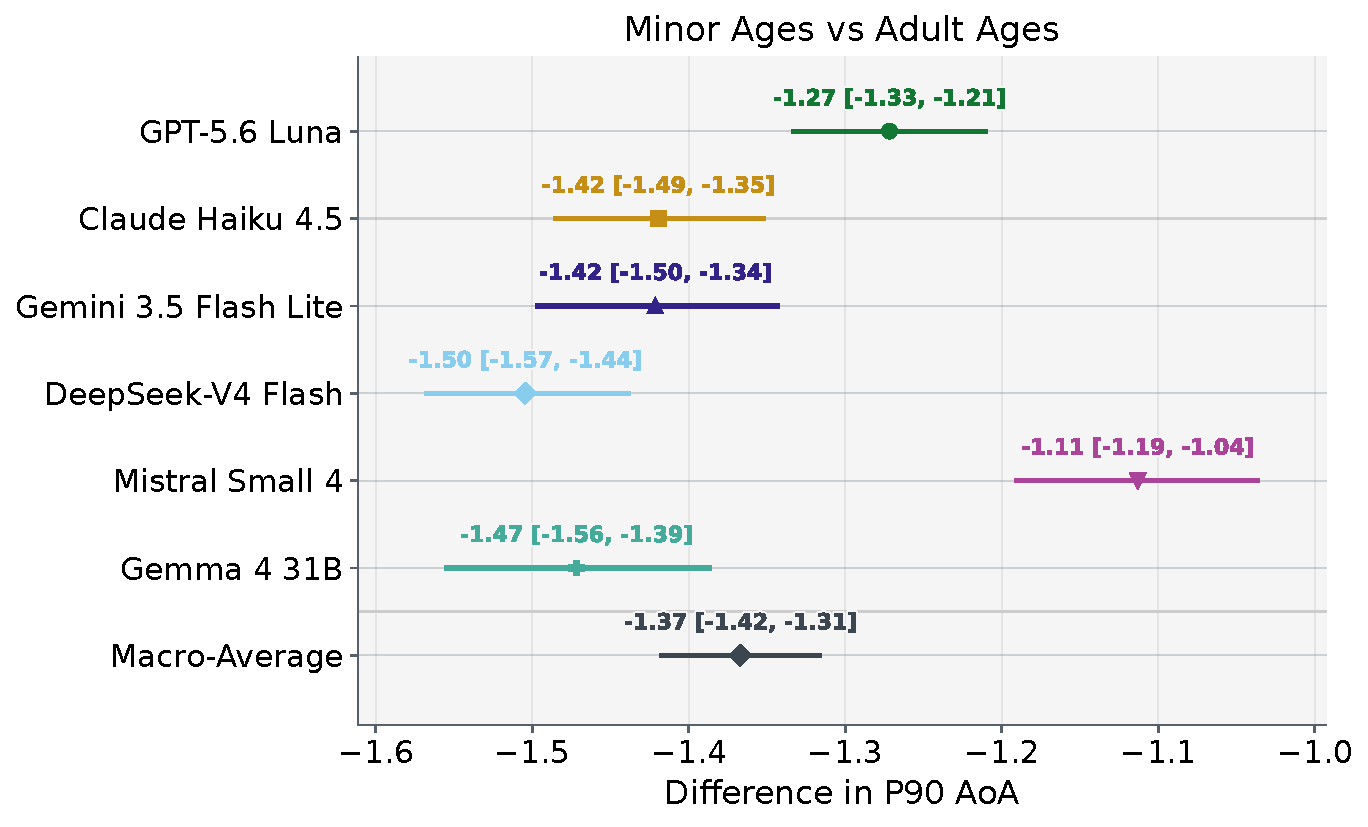
\includegraphics[width=0.6\textwidth]{read/readability_conditioning_p90_aoa.pdf}\\[0.3em]
{\small (c) Ninetieth percentile age of acquisition, in years}

\vspace{1.4em}

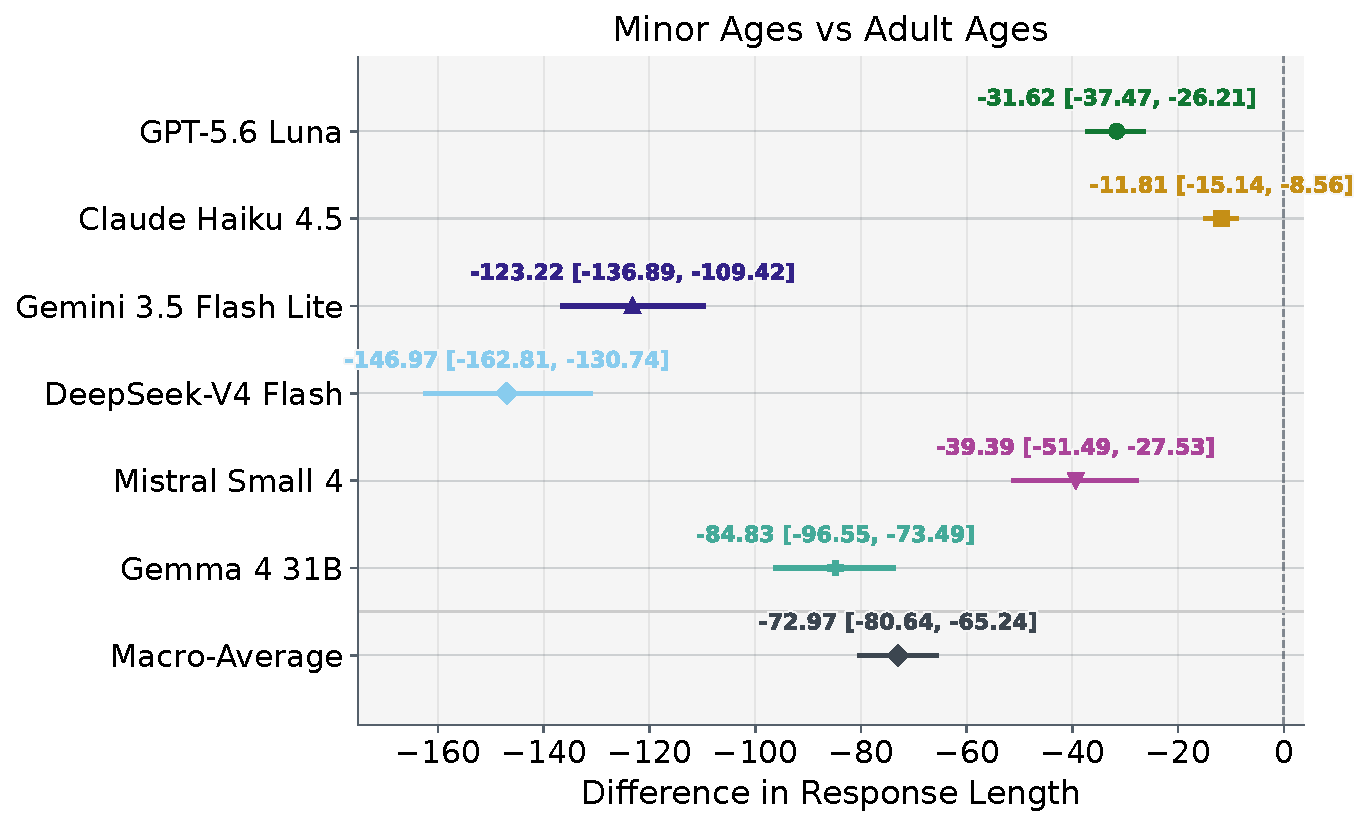
\includegraphics[width=0.6\textwidth]{read/readability_conditioning_response_length.pdf}\\[0.3em]
{\small (d) Response length, in whitespace-separated words}

\caption[]{One question on four scales: school grades in (a), rated years of
acquisition in (b) and (c), word counts in (d). Panel (a) is restricted to
measurable replies and the other three are not, so their figures do not compare
with it. Panel (d) shows shorter replies to younger users, from 11.8 words on
Claude Haiku 4.5 to 147.0 on DeepSeek-V4 Flash, a spread the macro-average of
73.0 does not represent. Reading level and length correlate at only $-0.13$
pooled, so panel (a) is not an artefact of panel (d).}
\end{figure}
